\section{W2: Process Control and Models}

\textbf{Defined Process Control}: A process with a well-defined set of steps. Almost like a function; take same inputs, get same outputs.

\textbf{Empirical Process Control}: A process that is continuously improved.

\textbf{Process Model}: A simplified description of the steps to achieve your goal.

\textbf{Formal SDLC Processes}

    \textbf{Waterfall}: Linear, sequential, non-iterative. Each phase must be completed before the next phase begins.

    \textbf{Incremental}: Breaks down the project into smaller, more manageable modules. Each module is developed and tested separately.

    \textbf{Prototyping/Rapid Prototyping}: Develop a working model of the system. Used to gather requirements.

    \textbf{Spiral}: Combines elements of both design and prototyping-in-stages. Each cycle involves a prototype to test.
    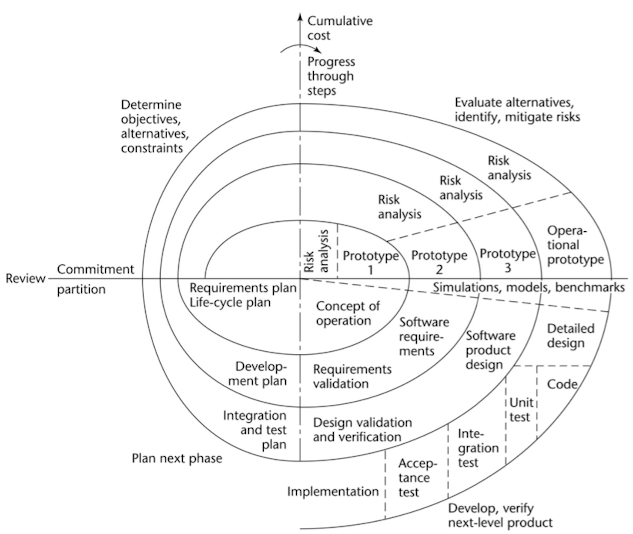
\includegraphics[width=\linewidth]{figs/SCR-20240605-oywi.png}


\textbf{Agile Family of Processes (2001)}

    \textbf{Agile Manifesto}: Individuals and interactions over processes and tools, working software over comprehensive documentation, customer collaboration over contract negotiation, responding to change over following a plan.

    \textbf{Agile Principles}: Customer satisfaction by rapid delivery of useful software, welcome changing requirements, deliver working software frequently, close, daily cooperation between business people and developers, projects are built around motivated individuals, face-to-face conversation is the best form of communication, working software is the primary measure of progress, sustainable development, attention to technical excellence and good design, simplicity, self-organising teams, regular adaptation to changing circumstances.

    \textbf{Agile Frameworks}

        \textbf{Kanban}: Visualise work, limit work in progress, focus on flow, make policies explicit, implement feedback loops, improve collaboratively.

        \textbf{eXtreme Programming (XP)}: Kent Beck developed the framework in late 90's. Pair programming. Intended to improve productivity and introduce checkpoints at which new customer requirements can be adopted.

        \textbf{Scrum (1986)}: Jeff Sutherland and Ken Schwaber presented paper on Scrum in a Conference in 1995. Everything is divided into timeframes.
        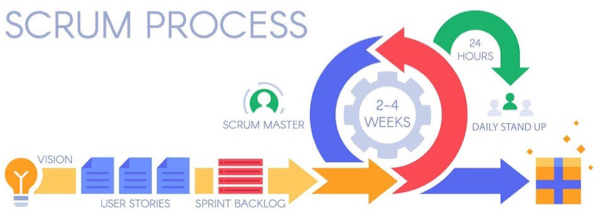
\includegraphics[width=\linewidth]{figs/SCR-20240605-payc.png}

        \textbf{PayPal Case Study}: They went from waterfall to agile.
